\documentclass{article}
\usepackage{graphicx} % Required for inserting images
\usepackage[spanish, english]{babel}
\usepackage[hidelinks]{hyperref}
\usepackage{makecell}
\usepackage[numbered,framed]{listings}
\usepackage{color} % red, green, blue, yellow, cyan, magenta, black, white
\usepackage{enumitem}
\usepackage{lmodern}
\usepackage{array}
\usepackage{float}
\usepackage{tabularx}
\usepackage{siunitx}
\usepackage{booktabs}
\usepackage{footnote}          % <— nuevo
\usepackage{siunitx}
\usepackage{inputenc}
\usepackage{threeparttable}
\usepackage{tikz}       % Diagrama en capas (cubo)
\usepackage{footmisc}   % Mejor gestión de notas a pie de página (opcional)
\definecolor{mylilas}{RGB}{170,55,241}
\definecolor{backcolour}{rgb}{0.92,0.95,0.95}

\usepackage{longtable}
\usepackage{geometry}
\usepackage{lipsum}

\usepackage{listings}
\usepackage{xcolor}
\lstdefinestyle{custom}{
    backgroundcolor=\color{black!5},           % Fondo más sutil (gris muy claro)
    basicstyle=\ttfamily\footnotesize,         % Fuente monoespaciada más pequeña y profesional
    keywordstyle=\color{blue!70!black},        % Palabras clave en azul oscuro
    stringstyle=\color{orange!80!black},       % Cadenas en naranja suave
    commentstyle=\color{gray!50},              % Comentarios en gris claro
    numberstyle=\tiny\color{gray!40},          % Números de línea discretos
    numbers=left,                              % Números a la izquierda
    numbersep=10pt,                            % Espaciado entre números y código
    breaklines=true,                           % Romper líneas largas
    breakatwhitespace=true,                    % Romper solo en espacios
    frame=tb,                                  % Marco solo arriba y abajo (más elegante)
    framesep=5pt,                              % Espaciado interno del marco
    captionpos=b,                              % Título debajo
    showstringspaces=false,                    % No mostrar espacios en cadenas
    tabsize=4,                                 % Tamaño de tabulación
    escapeinside={(*@}{@*)},                   % Permitir escapar a LaTeX dentro del código
    morekeywords={app, def, return, send, register_blueprint, SocketIO} % Palabras clave adicionales
}


\newcolumntype{L}[1]{%
  >{\setlength\parindent{1em}% sangría primera línea
    \raggedright\arraybackslash}%
  p{#1}%
}

\begin{document}



% Configurando la numeración arábiga desde el inicio
\pagenumbering{arabic}

% Creando la portada
\begin{titlepage}
    \centering
    {
\includegraphics[width=0.9\textwidth]{Imagenes/Universidad-de-Valladolid.png}}\par
    {\bfseries\Large Escuela Técnica Superior de Ingenieros de Telecomunicación\par}
    \vspace{0.5cm}
    {\bfseries\itshape\Large Trabajo de Fin de Grado \par}
    \vspace{0.5cm}
    {\scshape Grado en Ingeniería de Tecnologías de Telecomunicación \par}
    \vspace{0.5cm}
    {\bfseries\scshape\Large Request To Pay frente a la domiciliación bancaria: propuesta de mejora e implementación de un prototipo. \par}
    \vspace{1.5cm}
    { Autor: \\}
    { Alonso Sandoval Martínez }\\
    \vspace{0.5cm}
    { Tutor:\\}
    { Federico Simmross Wattenberg }\\
    \vspace{1.5cm} {Valladolid, junio 2025 \par}
\end{titlepage}

% Configurando el idioma
\selectlanguage{spanish}  

% Añadiendo el índice justo después de la portada
\newpage
\tableofcontents

% Añadiendo los agradecimientos desde un archivo externo
\newpage
\cleardoublepage            % empieza en página nueva
\phantomsection
\addcontentsline{toc}{section}{Agradecimientos}

\thispagestyle{empty}       % sin cabecera ni número de página

\vspace*{\fill}             % empuja el bloque hacia el centro vertical
\begin{center}
\section*{Agradecimientos}

Agradezco, en primer lugar, la orientación y el seguimiento de mi tutor,  
cuya experiencia ha sido decisiva para completar este trabajo.

Extiendo mi gratitud a mi familia por su respaldo constante y a mis amigos  
por el apoyo práctico y la paciencia mostrada durante el desarrollo del proyecto.

Su ayuda conjunta ha permitido que este trabajo llegue a buen término.
\end{center}
\vspace*{\fill}             % completa el centrado vertical


% Añadiendo el resumen en español
\newpage
\phantomsection
\addcontentsline{toc}{section}{Resumen}

\thispagestyle{empty}
\section*{Resumen}

Este Trabajo de Fin de Grado (TFG) explora cómo mejorar los sistemas de cobro en Europa, comparando el método tradicional de domiciliación bancaria (SEPA Direct Debit o SDD) con una solución más moderna: el esquema Request To Pay (RTP). El SDD, aunque muy usado, tiene limitaciones como procesos lentos, necesidad de documentos físicos y riesgos de devoluciones, lo que lo hace poco práctico para el mundo digital actual, donde se busca rapidez y simplicidad. En cambio, el RTP permite a quien cobra enviar una solicitud de pago digital que el pagador puede aceptar o rechazar al instante, haciendo el proceso más rápido, seguro y eficiente.

El objetivo del TFG ha sido crear un prototipo que simule cómo funcionaría un proveedor de RTP. Este prototipo, desarrollado con herramientas como Node.js y una base de datos sencilla, muestra cómo se pueden gestionar solicitudes de pago en tiempo real, desde su creación hasta su aprobación o rechazo. Las pruebas realizadas confirman que el sistema funciona bien y resuelve problemas del SDD, como la lentitud y la falta de control inmediato.

Este trabajo no solo demuestra que el RTP puede ser una alternativa útil para modernizar los pagos, sino que también abre la puerta a mejoras futuras, como hacerlo más seguro o conectarlo con bancos reales. En resumen, el prototipo es un paso hacia un sistema de cobros más ágil y adaptado a las necesidades de hoy, con potencial para cambiar cómo manejamos las transacciones en Europa.



% Volviendo al español para el resto del documento
\selectlanguage{spanish} 


% Comenzando el cuerpo principal (numeración ya es arábiga)
\newpage

\section{Introducción}
\label{sec:Introduccion}

Para comprender el entorno actual de los pagos en Europa, conviene arrancar por la \emph{Single Euro Payments Area} (SEPA): un espacio comunitario en el que todos los pagos en euros se rigen por los mismos estándares técnicos y normas operativas, de modo que enviar dinero de un país a otro resulta tan ágil y claro como una transferencia nacional. SEPA estableció protocolos de mensajería comunes, armonizó los plazos de liquidación y fijó reglas uniformes de protección al usuario, creando la base sobre la que se despliegan hoy los servicios de pago más innovadores.

En los últimos diez años, la digitalización de los servicios financieros ha cambiado por completo cómo particulares y empresas gestionan sus transacciones dentro de ese marco SEPA. Las transferencias instantáneas, las API abiertas de los bancos y el auge del comercio electrónico han disparado la demanda de procesos de cobro que sean sencillos, transparentes y en tiempo real. No obstante, los instrumentos de pago tradicionales —tarjetas, transferencias convencionales o domiciliaciones— nacieron en un contexto muy distinto y todavía arrastran limitaciones que penalizan tanto la experiencia de usuario como la eficiencia operativa.

Aquí es donde entra en juego \emph{Request-to-Pay} (RTP). Este servicio de mensajería permite al beneficiario enviar al pagador una solicitud de pago digital estructurada, con todos los detalles (importe, concepto, vencimiento), y recibir en segundos una respuesta —aceptación, rechazo o aplazamiento— antes de iniciar el movimiento de fondos. RTP no sustituye los métodos de pago existentes, sino que actúa como una capa de orquestación sobre la infraestructura SEPA (y, en especial, los pagos inmediatos) y los canales de banca online, facilitando la conciliación, reduciendo la fricción en el cobro y modernizando la experiencia tanto para empresas como para consumidores.

\subsection{Motivación}
\label{subsec:Motivacion}

La domiciliación bancaria regulada por el esquema \textit{SEPA Direct Debit} (\textbf{SDD})\footnote{\textit{SEPA Direct Debit} es el instrumento paneuropeo de cargo en cuenta regulado por el \emph{European Payments Council}.} desde 2014, sigue siendo el método principal para cobros recurrentes en España. No obstante, su estructura, pensada para un entorno de procesos \emph{offline}—genera hoy inconvenientes que chocan con las demandas de inmediatez, seguridad y experiencia de usuario fluida que caracterizan la economía digital actual.

\subsubsection{Ineficiencias operativas detectadas}

Tras analizar la operativa SDD nacional se han identificado una serie de ineficiencias que afectan tanto a los usuarios como a las entidades participantes en el proceso de pago resumidas en los siguientes \textbf{5} puntos:
\begin{enumerate}[label=\textbf{\arabic*.}, leftmargin=0.75cm]
      \item \textbf{Modelo off-line y necesidad de mandato físico}\\
            El proceso de pago mediante el esquema SDD opera bajo un modelo offline, lo que implica una ausencia total de interacción en tiempo real entre las partes involucradas. Para iniciar el cobro, el deudor debe firmar y enviar un \textbf{mandato SEPA}\footnote{El mandato SEPA es un documento mediante el cual el deudor autoriza al acreedor a realizar cobros automáticos a través de la domiciliación bancaria.} en formato físico. Este documento debe ser conservado por el acreedor durante toda la duración del contrato y hasta 14 meses después de la última transacción realizada. Aunque la digitalización ha avanzado en muchos ámbitos, aún no existe un estándar único y interoperable para los \textbf{eMandates}\footnote{Un eMandate es la versión electrónica del mandato SEPA, que permite autorizar cobros de manera digital.}, lo que lleva a que cada entidad bancaria implemente su propio sistema. Esta falta de uniformidad genera inconsistencias y dificulta la estandarización del proceso.
            \textbf{Consecuencias}:
      \begin{itemize}
            \item Fricciones significativas en los procesos de venta digital, ya que los usuarios deben completar pasos adicionales que rompen con la inmediatez esperada en el comercio electrónico actual.
            \item Costes operativos considerables asociados a la gestión administrativa, como el archivado, las auditorías y el mantenimiento de los mandatos físicos.
            \item Riesgos legales y financieros en caso de disputa, como devoluciones costosas o conflictos prolongados con los deudores, debido a la ausencia de un mandato válido.
      \end{itemize}

  \item \textbf{Derecho a devolución prolongado}\\
        El esquema SDD otorga al deudor un derecho a devolución excepcionalmente amplio, lo que genera incertidumbre en la gestión de los ingresos por parte de los acreedores. En el caso de un \emph{cobro autorizado}, el deudor puede solicitar la devolución del importe sin necesidad de justificar su decisión durante un periodo de \textbf{ocho semanas}, bajo la política conocida como \emph{“no-questions-asked”}. Por otro lado, si el cobro se clasifica como \emph{no autorizado} —por ejemplo, si el banco emisor no puede probar la existencia de un mandato válido—, el plazo para reclamar se extiende hasta \textbf{trece meses}.
        
        \textbf{Consecuencias}:
        \begin{itemize}
          \item Notable inseguridad para los acreedores, quienes deben mantener reservas de liquidez y provisiones contables para cubrir posibles devoluciones tardías.
          \item Facilitación de prácticas como el \emph{friendly fraud}\footnote{El \emph{friendly fraud} ocurre cuando un usuario consume un bien o servicio y, posteriormente, solicita una devolución sin justificación, aprovechando las políticas de devolución laxas.}, donde los deudores reclaman reembolsos injustificados tras haber recibido el producto o servicio.
          \item Impacto directo en la rentabilidad de las empresas debido a las devoluciones inesperadas.
        \end{itemize}

  \item \textbf{Ciclos de cobro lentos}\\
        Los tiempos de procesamiento en el esquema SDD son significativamente prolongados, lo que compromete tanto la eficiencia operativa como la experiencia del usuario. En el esquema \textsc{Core}\footnote{El esquema \textsc{Core} es el estándar de domiciliación bancaria SEPA utilizado para pagos entre empresas y consumidores.}, el acreedor debe enviar la orden de cobro al banco con una antelación de \textbf{D-5 días} para la primera domiciliación y de \textbf{D-2 días} para las domiciliaciones recurrentes. A esto se suman \textbf{dos días adicionales} para la liquidación interbancaria. En total, el proceso puede demorar entre seis y ocho días naturales desde que se solicita el cobro hasta que se confirma el abono, un plazo incompatible con las expectativas de inmediatez en la venta de bienes o servicios digitales.
        
        \textbf{Consecuencias}:
        \begin{itemize}
          \item Afectación en la planificación financiera de las empresas, ya que los ingresos no están disponibles de manera inmediata, generando una tesorería imprevisible.
          \item Riesgo de prestar servicios o entregar productos sin la certeza de que el pago se completará con éxito.
          \item Pérdidas económicas significativas debido a la falta de confirmación inmediata del pago.
        \end{itemize}

  \item \textbf{Costes y complejidad de las R-transactions}\footnote{Transacciones de rechazo, devolución o reembolso asociadas a pagos fallidos o no autorizados.}\\
        Las \textbf{R-transactions} representan una fuente notable de complicaciones y costes adicionales. Estas transacciones se clasifican mediante diversos códigos, cada uno asociado a un flujo y reglas específicas, lo que dificulta su gestión y seguimiento. Los acreedores deben dedicar recursos a identificar las causas de cada R-transaction y aplicar las medidas correctivas correspondientes, un proceso que frecuentemente requiere intervención manual debido a la falta de automatización.
        
        \textbf{Consecuencias}:
        \begin{itemize}
          \item Necesidad de equipos especializados en conciliación y recobro, incrementando los costes operativos.
          \item Reducción de la eficiencia general del sistema debido a la complejidad de los procesos.
          \item Posibilidad de errores o retrasos que afectan la productividad y la confianza en el esquema SDD.
        \end{itemize}

  \item \textbf{Ausencia de autorización fuerte (\textsc{SCA})}\footnote{La SCA (Strong Customer Authentication) es un requisito de seguridad establecido por la directiva PSD2, que exige la verificación del usuario mediante al menos dos factores de autenticación.}\\
        El esquema SDD se basa en un consentimiento previo otorgado mediante el mandato SEPA, pero no incorpora la \textbf{autorización fuerte del cliente (SCA)} en el momento de cada transacción. Una vez firmado el mandato, los cobros se ejecutan automáticamente sin que se solicite al deudor una autenticación adicional para cada operación.
        
        \textbf{Consecuencias}:
        \begin{itemize}
          \item Elevado riesgo de disputas por cargos no autorizados, lo que puede derivar en conflictos y devoluciones.
          \item Pérdida de una oportunidad clave para fortalecer la seguridad y la confianza en el proceso de cobro mediante métodos de autenticación modernos.
        \end{itemize}
\end{enumerate}

% Conclusión
\paragraph{En conclusión.} Estas ineficiencias tienen un gran impacto en la operativa y la competitividad de las empresas y entidades financieras que lo utilizan y se traducen en:

\begin{itemize}[leftmargin=0.45cm]
  \item Una \textbf{estructura de costes elevada}, derivada de la alta frecuencia de devoluciones y la necesidad de personal especializado para gestionarlas, lo que incrementa los gastos operativos.
  \item \textbf{Liquidez incierta}, ya que los ingresos no se confirman de inmediato y pueden ser revertidos incluso meses después de haberse registrado, dificultando la gestión financiera.
  \item Un \textbf{freno al desarrollo de la economía digital}, puesto que el SDD no está diseñado para ofrecer experiencias de pago instantáneas y fluidas, como las que proporcionan métodos alternativos como las tarjetas de crédito, los monederos electrónicos o plataformas como Bizum.
\end{itemize}

\subsubsection{Oportunidad de un esquema Request-to-Pay}
El estándar \textit{SEPA Request-to-Pay} (\textbf{SRTP})\footnote{Iniciativa del European Payments Council que define un flujo de solicitud (\textit{request}) y aceptación de pagos en tiempo real, apoyado en mensajería \textbf{ISO 20022} y siendo independiente del instrumento de liquidación posterior.} abroda de manera efectiva las limitaciones técnicas y operativas del SDD, ofreciendo una laternativa más ágil y adaptada al entorno digital.

A continuación se describen las principales ventajas del SRTP frente al SDD:

\begin{enumerate}[label=\alph*)]
  \item \textbf{Autenticación reforzada y consentimiento digital inmediato}\\
      El SRTP reemplaza el mandato físico del SDD por una solicitud de pago que el deudor aprueba directamente desde su banca en línea o wallet digital mediante SCA. Este proceso genera una prueba eléctronica de consentimiento, firmada y resgistrada en el sistema del PSP del pagador, eliminando la dependencia de documentos en papel y simplificando la gestión de autorizaciones.

  \item \textbf{Irrevocabilidad y mitigación de fraude \emph{post-servicio}}\\
      Una vez aceptada la solicitd, el pago se ejecuta mediante SCT Inst\footnote{\textsc{SCT Inst}: transferencia inmediata SEPA con liquidación en menos de10 s.}. A diferencia del SDD que permite devoluciones automáticas en plazos amplios, el SRTP no admite reversiones sin causa justificada. Esto minimiza el riesgo de textbf{fraude amistoso}-donde el deudor reclama devoluciones tras recibir un servicio- y reduce la necesidad de provisiones por impagos.

  \item \textbf{Liquidez \emph{real-time} y conciliación automática}\\
      Con fondos disponibles en menos de 10 segundos, las empresas pueden gestionar su tesorería con mayor precisión. Además, el uso de identificadores únicos y referencias estructuradas según el estándar ISO 20022 asegura que la información del pago se transmita íntegramente de extremo a extremo, permitiendo una conciliación automática y eliminando los retrasos y errores típicos del SDD.

  \item \textbf{Simplificación operativa}\\
      El SRTP elimina las R-transactions, la custodia de mandatos físicos y las tareas administrativas asociadas. El flujo se reduce a dos mensajes principales -solicitud y aceptación-, con la opción de una transferenciua instantánea, ofreciendo una trazabilidad clara y directa.

  \item \textbf{Flexibilidad comercial y costes reducidos}\\
      Este esquema soporta cobros únicos, recurrentes o fraccionados a través de canales digitales como enlaces profundos, códigos QR o APIs. Al estar basado en SCT Inst, las comisiones bancarias son bastante menores a las de las tarjetas o la destión de devoluciones del SDD, lo que mejora la eficiencias y amplía su aplicabilidad en el comercio electrónico.
\end{enumerate}

En conjunto, el SRTP conserva los puntos fuertes del SDD pero los adapta a las necesidades actuales, proporcionando una solución más rápida, segura y eficiente. Al superar las ineficiencias del SDD se convierte en una herramienta clave para modernizar los sistema de pago en la zona SEPA y, en concreto, en España.
\vspace{0.5cm}

\begin{table}[h]
\centering
\caption{Comparativa entre SDD y SRTP con SCT Inst}
\label{tab:comparativa-sdd-srtp}
\renewcommand{\arraystretch}{1.2}
\begin{tabular}{@{}L{4.8cm}C{4.8cm}C{4.8cm}@{}}
\toprule
\textbf{Aspecto} & \textbf{SDD} & \textbf{SRTP (+ SCT Inst)} \\
\midrule
Autorización & Mandato off-line & Consentimiento digital (\textsc{sca}) \\
Plazo de devolución & 8 semanas / 13 meses & No aplica (irrevocable) \\
Disponibilidad de fondos & 5--8 días & Menos de 10 segundos \\
Coste operativo & Alto (mandatos, \textsc{r-codes}) & Bajo (mensajería ISO 20022) \\
Cobertura \emph{e-commerce} & Limitada & Amplia (API / móvil) \\
Riesgo de fraude & Medio-Alto (devoluciones) & Bajo (\textsc{sca} + irreversibilidad) \\
\bottomrule
\end{tabular}
\end{table}

\bigskip


\subsection{Objetivos}
\label{subsec:Objetivos}
El propósito central de este TFG es desarrollar un sistema de software que simule, de principio a fin, un proveedor del esquema SRTP. Este proyecto nace con la idea de abordar las limitaciones del SDD, explicadas anteriormente. Se quiere demostrar que el SRTP puede ser una solución moderna, ágil y segura para los pagos en Europa, alineada con la versión 4.0 del \textit{SRTP Scheme Rulebook} \cite{epc014} y las guías técnicas del European Payments Council (\textit{EPC137} y \textit{EPC164}) \cite{epc137,epc164}.

El sistema será un prototipo funcional que se pueda instalar fácilmente con \texttt{Docker Compose} y que ofrezca una API HTTP/JSON basada en el estándar \textit{OpenAPI 3.1}. Este prototipo debe cubrir las cuatro operaciones principales del flujo SRTP: crear una solicitud de pago (\textit{create}), rechazarla (\textit{reject}), responder a ella (\textit{response}) y cancelarla (\textit{cancel}). En resumen, queremos construir una herramienta que no solo funcione, sino que también sea práctica y fiel a las especificaciones del SRTP.

Para mantener el proyecto enfocado y medible, hemos definido los siguientes \textbf{objetivos específicos}:

\begin{enumerate}[leftmargin=0.75cm]
  \item \textbf{Desarrollar una API robusta y eficiente.} \\
        Implementar, usando \texttt{Node.js 20 LTS} y \texttt{Express}, un conjunto de \textit{endpoints} REST que garanticen alta disponibilidad. Además, incluir un sistema de notificaciones asíncronas mediante \texttt{Socket.IO} para que las actualizaciones lleguen en tiempo real, reflejando la inmediatez que el SRTP promete frente al lento SDD.

  \item \textbf{Garantizar seguridad y confianza.} \\
        Crear un módulo que gestione firmas digitales, sellado temporal y validación con certificados X.509 (\textit{QSeal}/\textit{QWAC}). Esto asegurará que el sistema cumpla con los requisitos de identificación, autenticación y autorización del \textit{API Security Framework} \cite{epc164}, protegiendo cada transacción y resolviendo la falta de autenticación fuerte del SDD.

  \item \textbf{Almacenar datos de forma sencilla y fiable.} \\
        Diseñar una base de datos ligera en \texttt{SQLite}, gestionada con \texttt{SQLAlchemy}, para guardar el estado de las operaciones y su auditoría. El modelo de datos estará alineado con los \textit{datasets} DS-02, DS-07 y DS-10 del \textit{Rulebook}, asegurando que todo esté bien organizado y traceable.

  \item \textbf{Asegurar la calidad con pruebas automatizadas.} \\
        Entregar una colección de pruebas en \texttt{Postman} y un flujo de integración continua en \texttt{GitHub Actions}. Estas pruebas verificarán la integración del sistema y validarán los esquemas JSON contra los estándares oficiales del EPC, garantizando que el prototipo funcione como se espera.

  \item \textbf{Documentar y planificar mejoras futuras.} \\
        Identificar cualquier diferencia entre las especificaciones del SRTP y nuestra implementación, explicando por qué ocurrieron. También propondremos una hoja de ruta clara para ajustar el sistema y hacerlo compatible con el \textit{Electronic Data Submission} (EDS) en el futuro, asegurando su relevancia a largo plazo.

\end{enumerate}

En definitiva, este TFG busca construir una solución práctica que demuestre el potencial del SRTP para superar las trabas del SDD, usando tecnologías modernas y un enfoque riguroso. Queremos que este prototipo no solo cumpla con los estándares técnicos, sino que también inspire confianza en una nueva forma de gestionar pagos en Europa.

\subsection{Fases y Métodos}
\label{subsec:FasesMetodos}
El TFG se ha estructurado en 3 fases principales:

\begin{description}
  \item[Fase 1 – Análisis y planificación]%
      En esta primera etapa se estudió el mundo de los pagos en la zona SEPA, revisando los documentos emitidos por el EPC para identificar las posibles mejoras que el RTP podría suponer.
      
      Luego, se estudiaron los casos de uso del RTP, identificando qué necesitan hacer los actores principales y se planificó el prototipo.
  \item[Fase 2 – Diseño e implementación]%
      Una vez claro el conexto, se comenzó a diseñar la estructura del prototipo definiendo los roles de los actores y cómo interactúan entre si.

      La implementación se ha llevado a cabo usando herramientas que se detallarán posteriormente.
  \item[Fase 3 – Pruebas y validación]%
      Por último, una vez implementado el prototipo se realizaron una serie de pruebas y comprobaciones para verificar que todo funciona correctamente, como veremos en otro apartado del documento.
\end{description}

\subsection{Medios necesarios empleados para el desarrollo}
\label{subsec:Medios}
\begin{itemize}
  \item \textbf{Software de desarrollo:}  
        \texttt{Node.js 20 LTS}, \texttt{Express 4}, \texttt{Socket.IO 4},
        \texttt{Sequelize 6}, \texttt{Jest}, \texttt{Postman v10},
        \texttt{Docker 24}, \texttt{Docker Compose v2},
        \texttt{Git} y \texttt{GitHub Actions}.
  \item \textbf{Herramientas de apoyo:}  
        \texttt{OpenSSL 3} para gestión de certificados,
        \texttt{toxiproxy} para pruebas de resiliencia,
        \texttt{Spectral OCI} para linting de especificaciones OpenAPI.
  \item \textbf{Documentación oficial:}  
        SRTP Scheme Rulebook v4.0 \cite{epc014},  
        SRTP related API Specifications v3.1 \cite{epc137},  
        API Security Framework v2.0 \cite{epc164},  
        ISO 20022 \emph{pacs/pain/camt},  
        directivas PSD2/eIDAS.
  \item \textbf{Hardware y S.O.:}  
        Portátil x86-64, 16 GB RAM, SSD 512 GB, Ubuntu 22.04 LTS, conexión
        simétrica de 300 Mbps; virtualización \texttt{Docker Desktop}.
  \item \textbf{Repositorios y control de versiones:}  
        Organización privada en GitHub; \texttt{branch protection} y
        \texttt{semantic-versioning}.
\end{itemize}
\newpage

%----------------------------------------------------------------------
% Antecedentes y estado del arte
%----------------------------------------------------------------------

\section{Antecedentes y estado del arte}
\label{sec:estado-arte}

\subsection{Evolución de los medios de pago hacia SEPA}
\label{subsec:evolucion-sepa}


El ecosistema europeo de pagos ha experimentado una profunda transformación en las últimas décadas, pasando de sistemas nacionales heterogéneos a un marco unificado bajo la iniciativa \textbf{SEPA}. Antes de SEPA, cada país operaba infraestructuras y normas propias para transferencias bancarias y adeudos, lo que complicaba los pagos transfronterizos dentro de Europa.  
Con la introducción del euro y el objetivo de un mercado único, surgió la necesidad de armonizar los instrumentos de pago. El Consejo Europeo impulsó la creación de SEPA a través del Reglamento (UE)~\num{260}/\num{2012}, que fijó la migración obligatoria a los nuevos esquemas paneuropeos de transferencia y adeudo en fechas límite (febrero de 2014 para la zona euro).  

Así, en \textit{2008} se lanzó el esquema \textbf{SEPA Credit Transfer} (\textbf{SCT}) para transferencias de crédito en euros, y en \textit{2009} el \textbf{SEPA Direct Debit} (\textbf{SDD}) para adeudos domiciliados. Estos esquemas sustituyeron progresivamente a los medios nacionales, unificando formatos (por ejemplo, el uso obligatorio de \emph{IBAN}) y reglas de funcionamiento en todos los países SEPA. Posteriormente, para atender las demandas de inmediatez, la transferencia instantánea \textbf{SCT~Inst} (\emph{SEPA Instant Credit Transfer}) entró en funcionamiento en \textit{2017}, permitiendo abonar al beneficiario en menos de \SI{10}{\second}. La implantación de SCT~Inst ha sido voluntaria hasta ahora, aunque recientemente la UE ha aprobado su obligatoriedad progresiva en 2025 para acelerar su adopción.  

En la actualidad, los esquemas SEPA (transferencias estándar e inmediatas, adeudos básicos y B2B) concentran la mayoría de pagos bancarios en euros dentro de Europa. Este salto hacia la unificación de pagos fue liderado por la propia industria bancaria europea. En \textit{2002} los bancos constituyeron el \textbf{European Payments Council} (EPC), órgano de autorregulación que diseña y gestiona los esquemas SEPA. El EPC publicó las primeras \emph{rulebooks} de SCT y SDD en 2008–2009, estableciendo estándares comunes de mensaje (\emph{ISO~20022}\footnote{ISO~20022: estándar internacional para el intercambio de mensajes financieros, basado en XML, empleado en los esquemas SEPA para definir las estructuras de datos de transferencias, adeudos, etc.}) y calendarios de liquidación. Cabe destacar que el EPC no es un organismo legislativo de la UE ni un regulador, sino una asociación del sector bancario que actúa de facto como ente normalizador: especifica las reglas de los esquemas utilizados por los \textbf{PSP} (\emph{Payment Service Providers} o proveedores de servicios de pago) y coopera con los bancos centrales para operar las infraestructuras de compensación. Gracias a esta colaboración público-privada, a partir de \textit{2014} se completó con éxito la migración de millones de pagos nacionales al formato SEPA, eliminando diferencias entre pagos domésticos y transfronterizos en euros.

\subsection{El papel del EPC en la estandarización y el surgimiento de Request-to-Pay}
\label{subsec:epc-rtp}

El \textbf{European Payments Council (EPC)} ha desempeñado un rol central en la estandarización de los instrumentos de pago SEPA. Tras la implementación de SCT y SDD, el EPC continuó explorando mejoras para la era digital, en línea con las iniciativas del Eurosistema para fomentar pagos electrónicos paneuropeos más eficientes. En noviembre de 2018, el \emph{Euro Retail Payments Board} (\textbf{ERPB})\footnote{ERPB: foro de alto nivel presidido por el BCE que reúne a autoridades y sector financiero para impulsar la integración y modernización de los pagos minoristas en Europa.} —órgano del BCE que orienta la estrategia de pagos minoristas— lanzó un llamado a la acción para desarrollar el concepto de \emph{Request to Pay} (R2P) como nuevo servicio en la zona SEPA.  

Atendiendo esta petición, el EPC creó un grupo de trabajo y comenzó a diseñar un esquema formal de Request to Pay durante 2019–2020. Tras una consulta pública, en noviembre de 2020 se publicó el primer \emph{SRTP Scheme Rulebook} (versión 1.0) y se abrió el registro de participantes. El esquema \textbf{SEPA Request-to-Pay (SRTP)} entró en vigor el \textit{15 de junio de 2021}, marcando un hito en la evolución de SEPA más allá de los instrumentos tradicionales. Al igual que SCT~Inst, la adhesión al esquema RTP es voluntaria; sin embargo, su desarrollo cuenta con fuerte apoyo institucional al considerarse un potenciador de los pagos instantáneos y digitales en Europa. El EPC continúa gestionando y actualizando el esquema (versión 4.0 en 2023), con la expectativa de que Request-to-Pay se integre gradualmente como componente clave del panorama de pagos europeos.

\subsection{Funcionamiento técnico de SEPA Request-to-Pay (SRTP)}
\label{subsec:funcionamiento-srtp}

\textbf{Request-to-Pay (RTP)} es un servicio de mensajería financiera que actúa como capa de solicitud previa al pago. A diferencia de los instrumentos tradicionales (transferencias o adeudos) que mueven fondos, RTP no mueve dinero por sí mismo: permite a un beneficiario (\emph{Payee}) enviar electrónicamente una solicitud de pago a un pagador (\emph{Payer}), quien puede aceptarla o rechazarla antes de iniciarse la transacción monetaria. El servicio funciona \emph{24 × 7} y añade al flujo de pago un intercambio estructurado de datos (importe, concepto, vencimiento, identidad de las partes, etc.) previo al envío de fondos.  

Los mensajes SRTP viajan en tiempo real formateados según ISO~20022\footnote{Las mensajes SRTP siguen las definiciones ISO~20022 específicas del esquema, permitiendo interoperabilidad con mensajes de pago \texttt{pacs}/\texttt{pain} de SCT/SCT~Inst.}, lo que facilita su integración con las plataformas SEPA existentes.

\paragraph{Modelo de cuatro esquinas.} SRTP adopta la clásica arquitectura \emph{4-corner model}:

\begin{figure}[H]
  \centering
  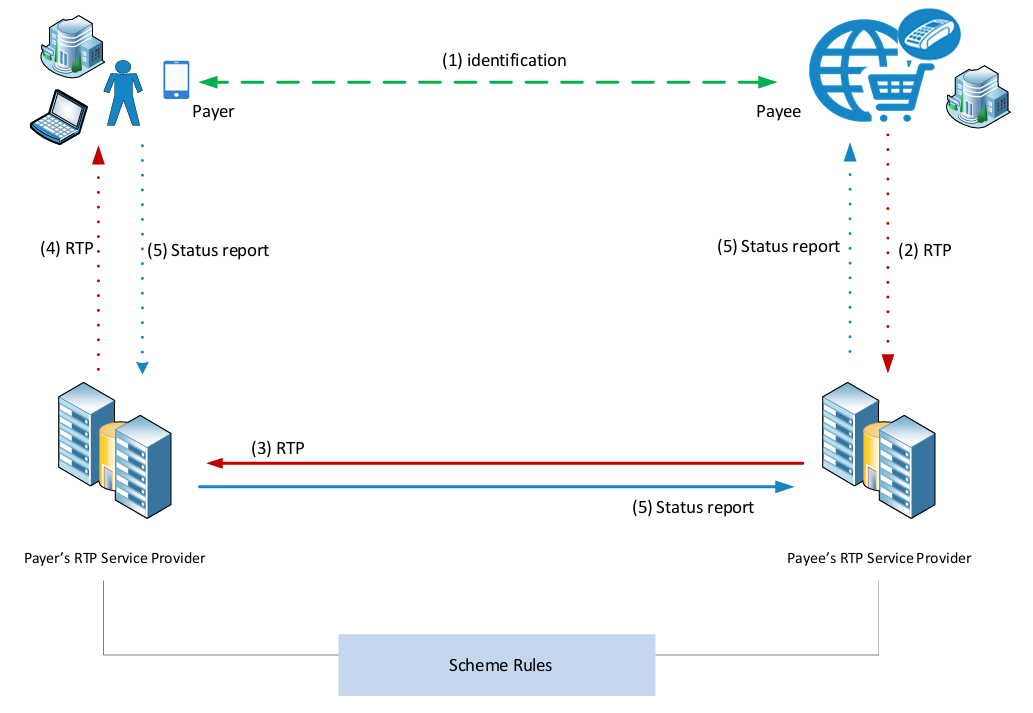
\includegraphics[width=0.8\textwidth]{Imagenes/4CornerModel.png}
  \caption{4CornerModel}
  \label{fig:4corner}
\end{figure}

\begin{table}[htbp]
  \centering
  \renewcommand{\arraystretch}{1.2} % aumenta un poco la altura de las filas
  \caption{Pasos del flujo del esquema SEPA Request-to-Pay (SRTP) y su descripción}
  \label{tab:srtp-steps-a}
  \begin{tabularx}{\textwidth}{@{} >{\bfseries}l  X @{}}
    \toprule
    Paso  & Descripción \\
    \midrule
    1.\ Identificación
      & Una primera interacción que establece la comunicación entre pagador y beneficiario. \\
    2.\ Envío de la SRTP al PSP del beneficiario
      & El beneficiario envía la solicitud de pago SRTP a su PSP, incluyendo todos los datos esenciales del esquema (importe, concepto, vencimiento…). \\
    3.\ Transmisión al PSP del pagador
      & El PSP del beneficiario reenvía la SRTP al PSP del pagador. \\
    4.\ Presentación al pagador
      & La solicitud se muestra al pagador en el canal acordado (app móvil, web, etc.), permitiendo que revise los detalles. \\
    5.\ Informe de estado
      & El resultado (aceptación o rechazo) se comunica de vuelta al beneficiario mediante los PSP correspondientes. \\
    \bottomrule
  \end{tabularx}
\end{table}

La Operational Scheme Manager (OSM) es el elemento central que mantiene vivo y accesible a todo el ecosistema SRTP. Es un gran directorio seguro y siempre actualizado, gestionado por el EPC, donde quedan registrados todos los PSP y demás actores autorizados: sus identificadores, los certificados TLS que usan para cifrar las comunicaciones, las claves de firma y las URLs de sus endpoints(puntos finales de API donde se reciben y se envían RTP). Gracias a la OSM, cada PSP puede, en cualquier momento, localizar de forma sencilla y confiable a otro PSP: comprueba automáticamente que el receptor está homologado, que su endpoint está operativo, y que la conexión será segura antes de intercambiar solicitudes o respuestas de pago.

Su misión va más allá de un simple directorio estático: la OSM supervisa y valida de forma continua la disponibilidad y el correcto funcionamiento de todos los endpoints adheridos, publica esta información en el EPC Directory Service (EDS) y notifica de inmediato cualquier incidencia. De este modo, se garantiza que las transacciones RTP fluyan sin interrupciones, con altos estándares de seguridad y cumplimiento de ISO 20022, y que todos los participantes puedan interoperar con total confianza.

En este TFG no se va a simular ni modelar este registro previo en la OSM, asumiremos que todos los actores se encuentran correctamente dados de alta en el directorio. Así, podremos centrarnos exclusivamente en las dinámicas de la solicitud, aceptación, rechazo yu cancelación de pagos, dando por hecho que el acceso a los endpoints y la homologación técnica ya están resueltos.

El flujo básico de un intercambio RPT es el aiguiente:
\newpage

\begin{figure}[H]
  \centering
  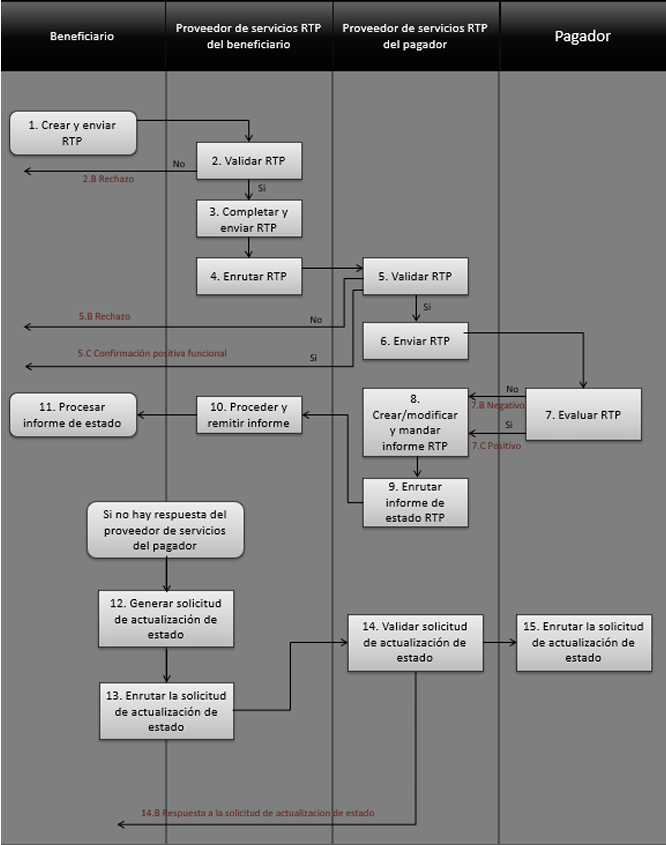
\includegraphics[width=0.95\textwidth, height=0.95\textheight, keepaspectratio]{Imagenes/Flujo.png}
  \label{fig:Flujo}
\end{figure}

\newcolumntype{L}[1]{%
  >{\setlength\parindent{1em}% sangría primera línea
    \raggedright\arraybackslash}%
  p{#1}%
}

\setlength{\tabcolsep}{10pt}
\renewcommand{\arraystretch}{1.5}
\begin{longtable}{|L{3cm}|p{12cm}|}
  \caption[Pasos del esquema SRTP]{Pasos del flujo del esquema SRTP y su descripción}
  \label{tab:srtp-steps-b} \\

  \hline
  \textbf{Paso/Función} & \textbf{Descripción} \\
  \hline
  \endfirsthead % Encabezado para la primera página

  \hline
  \textbf{Paso/Función} & \textbf{Descripción} \\
  \hline
  \endhead % Encabezado para las páginas siguientes

  \hline
  \multicolumn{2}{|c|}{\textit{(continúa en la siguiente página)}} \\
  \hline
  \endfoot % Pie de página para todas las páginas excepto la última

  \hline
  \multicolumn{2}{|c|}{\textit{Fin de la tabla}} \\
  \hline
  \endlastfoot % Pie de página para la última página

  % Contenido de la tabla
  1 Crear y enviar RTP & El beneficiario crea el "SEPA Request to Pay" SRTP en el formato normalizado (en un formato acordado bilateralmente con su proveedor). Contiene todos los elementos obligatorios y elementos opcionales que puedan ajustarse al flujo en función de las condiciones comerciales. El beneficiario lo envía al proveedor de servicios SRTP del beneficiario. \\
  \hline
  2 Validar RTP & El proveedor de servicios SRTP del beneficiario realiza una primera validación del SRTP. Esto incluye, por ejemplo, validación técnica, de seguridad y de formato (por ejemplo, comprobación del IBAN). \\
  \hline
  2B Rechazo & Si la validación en el paso 2 no tiene éxito, el proveedor de servicios SRTP del beneficiario notifica al beneficiario el rechazo del SRTP, crea un informe de estado negativo y lo envía al beneficiario en el formato acordado con este. \\
  \hline
  3 Completar y enviar RTP & En caso de validación correcta en el paso 2, el proveedor de servicios SRTP del beneficiario enriquece el SRTP con los elementos necesarios para el enrutamiento en el espacio entre proveedores de servicios SRTP y añade un sello de tiempo. \\
  \hline
  4 Enrutar RTP & El SRTP se envía al proveedor de servicios SRTP del pagador en función de los mecanismos de enrutamiento establecidos por el PSP. \\
  \hline
  5 Validar RTP & El proveedor de servicios SRTP del pagador valida el SRTP, incluye la comprobación del identificador del pagador. Esto puede incluir la validación específica del pagador (por ejemplo, si el pagador ha optado por no participar en el servicio, el SRTP es rechazado por defecto). \\
  \hline
  5B Rechazo & Si la validación en el paso 5 no tiene éxito, el proveedor de servicios SRTP del pagador rechaza el SRTP. El proveedor de servicios SRTP del beneficiario y el beneficiario son informados de este rechazo mediante un código de motivo de no aceptación del RTP. \\
  \hline
  5C Confirmación positiva funcional & Después de una validación externa en el paso 5, el proveedor de servicios SRTP confirma al pagador que el proveedor de servicios SRTP ha completado con éxito el procedimiento beneficial. Esta confirmación es obligatoria solo en el caso de que el beneficiario o el proveedor de servicios SRTP no haya confirmado previamente la positividad funcional. \\
  \hline
  6 Enviar RTP & En el caso de validación correcta en el paso 5, el proveedor de servicios SRTP envía el documento SRTP al pagador en el formato acordado (el SRTP puede ser convertido en este paso). \\
  \hline
  7 Evaluar RTP & El pagador decide si aceptar o rechazar el SRTP, determinando el próximo curso de acción. \\
  \hline
  7B Positivo & Si el pagador decide aceptar el SRTP, se envía una respuesta positiva al proveedor de servicios SRTP por parte del pagador. \\
  \hline
  7C Negativo & Si el pagador rechaza el SRTP, se envía una respuesta negativa al proveedor de servicios SRTP por parte del pagador. \\
  \hline
  8 Crear/modificar y mandar informe RTP & El proveedor de servicios SRTP crea un informe informativo basado en la decisión del pagador. Si la decisión es negativa (7B/7C), el informe se envía de vuelta al pagador para su revisión. Si el SRTP ya ha sido aceptado o rechazado, surge un caso excepcional donde no se espera un acuse de recibo. El informe debe considerar la fecha de expiración del SRTP. En este caso, el proveedor de servicios SRTP es responsable de notificar al beneficiario la decisión del proveedor de servicios SRTP, incluyendo el código correspondiente. Como resultado, el beneficiario debe representar el SRTP o utilizar otro canal. \\
  \hline
  9 Enviar informe de estado & El proveedor de servicios SRTP envía un informe de estado actualizado (positivo o negativo) al pagador a través del mismo canal utilizado para el SRTP original, utilizando mecanismos establecidos para la actualización. \\
  \hline
  10 Proceder y remitir informe & El proveedor de servicios SRTP del beneficiario procesa el informe de estado recibido (positivo o negativo), informa al beneficiario y decide los pasos siguientes previo acuerdo con el beneficiario. \\
  \hline
  11 Procesar informe de estado & El beneficiario ejecuta las acciones finales tras la recepción del informe de estado: actualización del estado final del registro SRTP, preparación del pago SRTP conciliación, etc. \\
  \hline
  12 Generar solicitud de actualización de estado & El beneficiario y el proveedor de servicios SRTP del beneficiario pueden enviar una Solicitud de Actualización de Estado si no se ha recibido respuesta hasta la Fecha/Hora de Expiración. \\
  \hline
  13 Enrutar la solicitud de actualización de estado & La solicitud de actualización de estado al proveedor de servicios SRTP del pagador se enruta a través de la misma vía utilizada para el SRTP original basándose en los mecanismos de enrutamiento establecidos. \\
  \hline
  14 Validar solicitud de actualización de estado & Tras la recepción de la solicitud de actualización de estado, el Proveedor de Servicios SRTP del pagador comprueba la validez de la Solicitud. \\
  \hline
  14B Respuesta a la solicitud de actualización de estado & El Proveedor de Servicios SRTP del pagador responde al proveedor de servicios SRTP del beneficiario y, si procede (a través del proveedor de servicios SRTP del beneficiario), al beneficiario (por ejemplo, respuesta del SRTP original no recibida, el pagador aún no ha respondido, etc.). \\
  \hline
  15 Enrutar la solicitud de actualización de estado & En caso de que el pagador aún no haya respondido al SRTP inicial, el proveedor de servicios SRTP del pagador puede enviar la solicitud de actualización de estado al Pagador. \\
  \hline
\end{longtable}

Hay algunos detalles acerca del esquema que conviene aclarar:
\begin{enumerate}
  \item \textbf{Rechazo de un SRTP o una Solicitud de Cancelación (Reject)} \\
        Un "Reject" se produce cuando un SRTP o una Solicitud de Cancelación no es aceptada antes de ser enviada al siguiente participante en la cadena de pago. El mensaje de rechazo sigue la misma ruta que el SRTP original sin modificar ningún dato, y se incluye un registro con los detalles necesarios para asegurar un rastro de auditoría. Además, el mensaje de rechazo lleva un código de motivo que explica la razón del rechazo. La identificación del SRTP original se hace mediante la referencia única incluida por el proveedor de servicios del receptor. Los rechazos se envían de manera instantánea por el proveedor de servicios SRTP que no puede procesar la solicitud, y estos rechazos pueden ser generados automáticamente en función de comprobaciones técnicas o comerciales, sin intervención del pagador.

  \item \textbf{Respuestas a un SRTP (positiva o negativa)} \\
        Cuando un pagador responde a un SRTP, puede aceptar (respuesta positiva) o rechazarlo (respuesta negativa). En ambos casos, el mensaje sigue la misma ruta que el SRTP original, sin alterar los datos, y se envía instantáneamente entre los proveedores de servicios SRTP. Las respuestas negativas incluyen un código de motivo que especifica la razón del rechazo, mientras que las respuestas positivas simplemente confirman la aceptación de la solicitud. Como en el caso de los rechazos, se mantiene un registro detallado de los datos relevantes para asegurar la trazabilidad del proceso y la transparencia en la comunicación entre los proveedores de servicios.

  \item \textbf{Solicitud de Cancelación del SRTP} \\
        Una “Request for cancelation” RfC puede ser iniciada por el y se transmite al pagador a través de los proveedores de servicios SRTP. La solicitud sigue la misma ruta que el SRTP original, sin modificar los datos, y debe incluir un código de motivo (atributo AT-R106) que justifique la cancelación. Esta solicitud puede realizarse hasta la fecha de expiración del SRTP, a menos que ya haya sido rechazado, cancelado o expirado. El proveedor de servicios SRTP del pagador verifica la validez de la solicitud antes de reenviarla, y si no se puede procesar, envía una respuesta negativa. Si la cancelación se ejecuta correctamente, el proveedor del pagador envía una respuesta positiva de manera instantánea, manteniendo siempre un registro para garantizar la trazabilidad del proceso.
\end{enumerate}
%%%%%%%%%%%%%%%%%%%%%%%%%%%%%%%%%%%%%%%%%%%%%%%%%%%%%%%%%%%%%%%%%%%%%%%%%%%%%%%%%%%%%%%%%%%%%%%%%%%%%%%%%%%%%%%%%%
%%%%%%%%%%%%%%%%%%%%%%%%%%%%%%%%%%%%%%%%%%%%%%%%%%%%%%%%%%%%%%%%%%%%%%%%%%%%%%%%%%%%%%%%%%%%%%%%%%%%%%%%%%%%%%%%%%
\paragraph{Casos de uso representativos.}
El \textbf{SEPA Request-to-Pay} se concibió como un servicio versátil, capaz de cubrir desde pagos cotidianos de bajo valor hasta cobros empresariales complejos. No obstante, el caso de uso considerado más transformador—y sobre el que se centra este TFG—es la \emph{sustitución del adeudo directo SEPA (SDD) en pagos recurrentes}. Aun así, existen otros escenarios relevantes que merece la pena describir para contextualizar el alcance potencial de SRTP.

\begin{enumerate}
    \item \textbf{Punto de Venta Físico (POS)}
    \begin{itemize}
        \item \textbf{Descripción:} Este caso de uso de Request to Pay se emplea en tiendas físicas, donde el payee (el comercio) envía una solicitud de pago al payor (el cliente) utilizando un código QR o una tecnología NFC (Near Field Communication). Al escanear el código QR con su móvil o usar NFC en la terminal de pago, el cliente es redirigido a su aplicación bancaria para autorizar el pago de manera inmediata.
        \item \textbf{Proceso de Identificación:}
        \begin{itemize}
            \item \textit{Identificación del Payor:} El payor se autentica directamente en su aplicación bancaria, generalmente mediante su número de cuenta bancaria, número de tarjeta, o métodos de autenticación biométrica o PIN, según lo permita la aplicación del banco.
            \item \textit{Identificación del Payee:} El payee está identificado en el sistema mediante un ID de comercio asociado a la terminal de pago o al código QR/NFC escaneado por el cliente. Estos elementos proporcionan los datos necesarios para vincular la solicitud de pago al comercio correspondiente.
        \end{itemize}
        \item \textbf{Proceso de Pago:}
        \begin{itemize}
            \item El cliente escanea el código QR o se conecta mediante NFC a la terminal de pago.
            \item La aplicación bancaria del cliente recibe la solicitud de pago con el monto y la referencia.
            \item El cliente revisa la información y autoriza el pago, un proceso rápido y conveniente, crucial en entornos físicos donde la velocidad es esencial.
        \end{itemize}
        \item \textbf{Diferencias Clave:}
        \begin{itemize}
            \item La rapidez y conveniencia son fundamentales en este caso de uso. El proceso de identificación y autorización es sencillo y rápido, requiriendo solo la confirmación del cliente a través de su banco, típicamente con autenticación biométrica o PIN.
            \item Es ideal para transacciones de bajo valor donde la experiencia del cliente es un factor determinante.
        \end{itemize}
    \end{itemize}

    \item \textbf{Comercio Electrónico (E-commerce)}
    \begin{itemize}
        \item \textbf{Descripción:} En este caso, el payee (el comercio electrónico) envía una solicitud de pago al payor (el cliente) durante el proceso de checkout o mediante un enlace de pago enviado a través de una aplicación bancaria o correo electrónico. El cliente es redirigido a su aplicación bancaria, donde debe autenticarse y revisar los detalles antes de aprobar el pago.
        \item \textbf{Proceso de Identificación:}
        \begin{itemize}
            \item \textit{Identificación del Payor:} La identificación implica un proceso de autenticación multifactor (por ejemplo, contraseña, token de seguridad o autenticación biométrica) para garantizar la seguridad de la transacción, realizado en la aplicación bancaria o la página de pago del comercio.
            \item \textit{Identificación del Payee:} El payee se identifica mediante un ID de comercio electrónico que incluye su nombre comercial, identificador fiscal, número de cuenta o un identificador único en la plataforma de pagos.
        \end{itemize}
        \item \textbf{Proceso de Pago:}
        \begin{itemize}
            \item El cliente recibe la solicitud de pago a través de un enlace en el checkout o en su aplicación bancaria.
            \item El cliente se autentica en su aplicación bancaria, revisa el monto, la referencia y los detalles del comerciante, y aprueba el pago.
            \item Una vez validada, el dinero se transfiere de manera segura.
        \end{itemize}
        \item \textbf{Diferencias Clave:}
        \begin{itemize}
            \item A diferencia del punto de venta físico, el proceso en comercio electrónico es más lento debido a la autenticación adicional y la revisión en línea.
            \item La seguridad es prioritaria, dado el mayor riesgo de fraude en transacciones digitales.
        \end{itemize}
    \end{itemize}

    \item \textbf{Facturación Electrónica (E-invoicing)}
    \begin{itemize}
        \item \textbf{Descripción:} Común en empresas que envían facturas electrónicas, el payee (la empresa emisora) envía una solicitud de pago con los detalles de la factura al payor (el cliente). El cliente recibe la solicitud en su correo electrónico o aplicación bancaria, pudiendo revisar los detalles antes de decidir cuándo pagar.
        \item \textbf{Proceso de Identificación:}
        \begin{itemize}
            \item \textit{Identificación del Payor:} El payor se identifica mediante su número de cliente, correo electrónico o número de cuenta bancaria vinculado a la empresa emisora.
            \item \textit{Identificación del Payee:} El payee se identifica por su NIF (Número de Identificación Fiscal) o un ID de facturación electrónica único, asegurando la verificación de la entidad receptora.
        \end{itemize}
        \item \textbf{Proceso de Pago:}
        \begin{itemize}
            \item El cliente recibe la factura y la solicitud de pago por correo o notificación bancaria.
            \item Tras validar la información, autoriza el pago a través de su aplicación bancaria, completando la transacción.
        \end{itemize}
        \item \textbf{Diferencias Clave:}
        \begin{itemize}
            \item Ofrece flexibilidad, permitiendo al cliente revisar la factura antes de pagar.
            \item La identificación del payee incluye detalles fiscales, incrementando la seguridad en la validación.
        \end{itemize}
    \end{itemize}

    \item \textbf{Pagos Recurrentes}
    \begin{itemize}
        \item \textbf{Descripción:} Ideal para suscripciones o pagos periódicos (streaming, software en la nube, gimnasios), el payor autoriza la primera transacción para suscribirse. Los pagos posteriores se gestionan automáticamente según la periodicidad acordada, sin intervención adicional.
        \item \textbf{Proceso de Identificación:}
        \begin{itemize}
            \item \textit{Identificación del Payor:} El payor autoriza la primera transacción con autenticación en su aplicación bancaria (cuenta, contraseña o biométrica).
            \item \textit{Identificación del Payee:} El payee se identifica por su ID de suscripción y número de cuenta para configurar los pagos recurrentes.
        \end{itemize}
        \item \textbf{Proceso de Pago:}
        \begin{itemize}
            \item El cliente autoriza el pago inicial.
            \item Los cobros posteriores se realizan automáticamente según la periodicidad (mensual, anual, etc.).
        \end{itemize}
        \item \textbf{Diferencias Clave:}
        \begin{itemize}
            \item Se distingue por la automatización tras la autorización inicial, reduciendo la intervención del cliente.
            \item La comodidad y la automatización son sus principales ventajas.
        \end{itemize}
    \end{itemize}

    \item \textbf{Pagos de Grandes Montos}
    \begin{itemize}
        \item \textbf{Descripción:} Utilizado en transacciones de alto valor (compras importantes, bienes de gran valor), este caso requiere métodos adicionales de autenticación para garantizar la seguridad.
        \item \textbf{Proceso de Identificación:}
        \begin{itemize}
            \item \textit{Identificación del Payor:} El payor usa autenticación robusta (OTP, tokens de seguridad o multifactor como PIN y biométrica) para validar la transacción.
            \item \textit{Identificación del Payee:} El payee es una entidad registrada con un identificador único (ID de comerciante), asegurando el destinatario correcto.
        \end{itemize}
        \item \textbf{Proceso de Pago:}
        \begin{itemize}
            \item El payor revisa el monto y autoriza el pago con autenticación adicional.
            \item Tras verificar la identidad, el pago se completa.
        \end{itemize}
        \item \textbf{Diferencias Clave:}
        \begin{itemize}
            \item Requiere autenticación más fuerte debido al alto riesgo de fraude en grandes sumas.
            \item La seguridad es el factor más crítico, priorizando la protección contra fraudes y errores.
        \end{itemize}
    \end{itemize}
\end{enumerate}
%%%%%%%%%%%%%%%%%%%%%%%%%%%%%%%%%%%%%%%%%%%%%%%%%%%%%%%%%%%%%%%%%%%%%%%%%%%%%%%%%%%%%%%%%%%%%%%%%%%%%%%%%%%%%%%%%%
%%%%%%%%%%%%%%%%%%%%%%%%%%%%%%%%%%%%%%%%%%%%%%%%%%%%%%%%%%%%%%%%%%%%%%%%%%%%%%%%%%%%%%%%%%%%%%%%%%%%%%%%%%%%%%%%%%
\subsection{RTP dentro del ecosistema de pagos: arquitectura en capas}
\label{subsec:cubo-pagos}

El ecosistema de pagos SEPA se puede describir mediante capas jerárquicas, desde los usuarios finales hasta las infraestructuras financieras que ejecutan las transacciones. A continuación se detallan las principales capas del modelo actual de pagos SEPA:

\begin{description}
  \item[\textbf{Capa de usuarios finales}] 
    En la capa más alta se encuentran el \emph{pagador} y el \emph{beneficiario}. Son quienes inician y reciben los pagos, respectivamente, ya sea personas o empresas involucradas en una transacción.

  \item[\textbf{Capa de iniciación o interacción}] 
    Es donde se produce la solicitud o autorización del pago a través de algún canal o interfaz. Por ejemplo, en pagos SEPA tradicionales el pagador suele autorizar una transferencia mediante la banca online o una aplicación móvil. En entornos de comercio electrónico o físico, esta capa correspondería al proceso de \emph{checkout} (por ejemplo, introduciendo datos en una pasarela de pago online o mediante un TPV/POS en tienda).

  \item[\textbf{Capa de proveedores de servicios de pago (PSP)}] 
    Aquí actúan las entidades financieras o PSP de cada parte. Típicamente, el banco del pagador y el banco del beneficiario son quienes ofrecen las cuentas bancarias y servicios de pago a sus clientes. Estas entidades facilitan la emisión y recepción de órdenes de pago en nombre de los usuarios finales.

  \item[\textbf{Capa de esquemas de pago}] 
    Es el conjunto de reglas y estándares comunes que permiten la interoperabilidad entre todos los PSP. En SEPA, por ejemplo, existen los esquemas de transferencia crediticia (SCT, SCT Inst) y adeudo directo (SDD), definidos por el European Payments Council (EPC). Cada esquema asegura que, independientemente del banco involucrado, un pago en euros siga las mismas normas y formatos. Un esquema de pago no es el movimiento del dinero en sí, sino el conjunto de reglas, mensajes e infraestructura técnica que orquesta cómo se inician y gestionan esos pagos.

  \item[\textbf{Capa de infraestructuras de compensación}] 
    Son las plataformas interbancarias que procesan las transacciones según las reglas del esquema. Estas infraestructuras se encargan de intercambiar las órdenes de pago entre el banco emisor y el banco receptor, aplicando compensación multilateral si procede.

  \item[\textbf{Capa de liquidación}] 
    Es la capa más baja, donde se realiza la liquidación final de fondos entre bancos. Normalmente ocurre en los bancos centrales u organismos de compensación: por ejemplo, las obligaciones netas resultantes de muchas transacciones SEPA pueden liquidarse en TARGET2 (sistema del Banco Central Europeo). En pagos inmediatos, la liquidación suele ser casi en tiempo real (por ejemplo, mediante TIPS que liquida cada operación al momento en cuentas del banco central).
\end{description}

\begin{figure}[H]
  \centering
  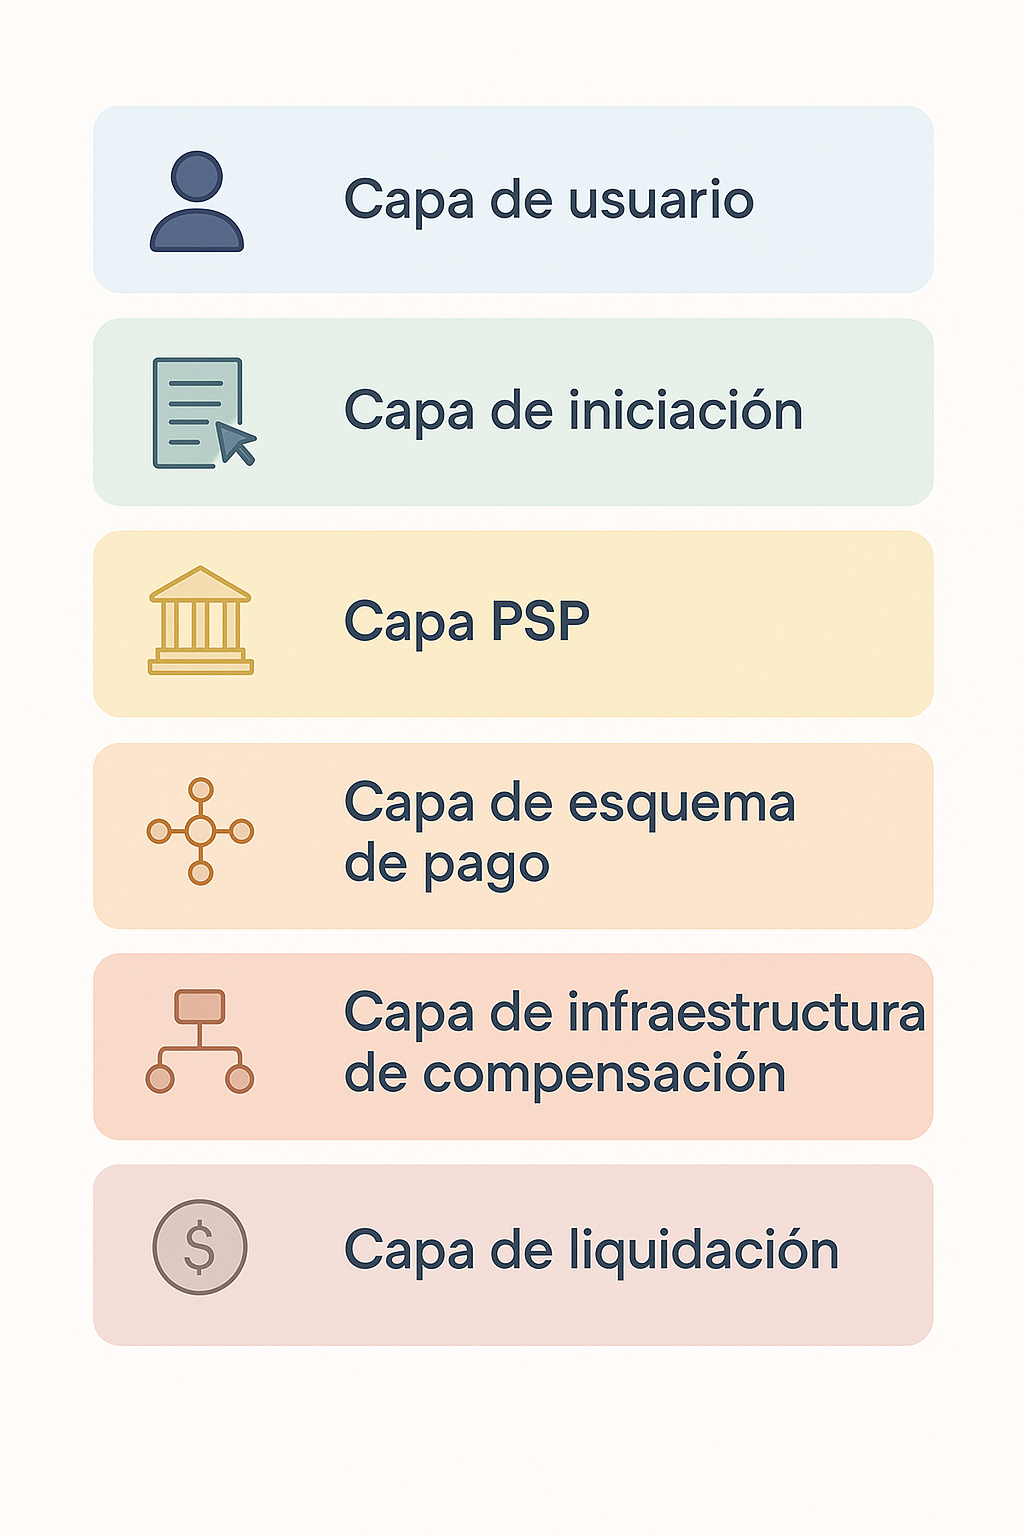
\includegraphics[width=0.5\textwidth]{Imagenes/esq1.png}
  \caption{Layer}
  \label{fig:Esquema por capas}
\end{figure}

Esta arquitectura por capas garantiza que un pago iniciado por un usuario en un banco pueda llegar a otro usuario en distinto banco de forma segura, eficiente e interoperable en toda la zona euro. Cada capa agrega funciones específicas: los usuarios generan órdenes, los PSP las gestionan, los esquemas proporcionan las reglas comunes, y las infraestructuras las ejecutan y asientan los fondos en última instancia.

RTP es un nuevo servicio/esquema incorporado en la arquitectura SEPA que se sitúa principalmente en la capa de esquema de pago, actuando como una capa adicional de mensajería sobre los instrumentos de pago existentes.

%----------------------------------------------------------------------
\subsubsection*{Ejemplo comparado: pago con tarjeta vs.\ RTP}

Como muestra el esquema comparativo, los pagos con tarjeta (ej.\ Visa/Mastercard) históricamente han operado con una arquitectura de funciones similar a la de SEPA, pero con diferencias en los actores y procesos de cada capa:

\begin{description}
  \item[\textbf{Usuarios (pagador/beneficiario)}]
    En tarjetas, el pagador es el \emph{titular de la tarjeta} y el beneficiario es el \emph{comercio} que recibe el pago. En esencia es equivalente al ordenante y beneficiario de una transferencia, con la diferencia de que el pagador utiliza un instrumento distinto (su tarjeta en lugar de una cuenta bancaria directa).

  \item[\textbf{PSP / entidades}]
    En el modelo de cuatro partes de las tarjetas interviene el \emph{banco emisor} (emite la tarjeta al pagador) y el \emph{banco adquirente} (procesa pagos para el comerciante). Estos roles son análogos a la entidad del pagador y del beneficiario en SEPA, pero en el mundo tarjeta suelen implicar acuerdos específicos (p.\,ej.\,el comerciante contrata un adquirente para aceptar Visa/Mastercard). En cambio, en SEPA cualquier banco puede enviar o recibir transferencias para un cliente sin acuerdos individuales con cada comercio, ya que todos siguen el esquema común.

  \item[\textbf{Esquema de pago}]
    Las tarjetas operan bajo esquemas propietarios como Visa, Mastercard, etc., que definen reglas, formatos de mensajes (p.\,ej.\ mensajes de autorización y liquidación) y que actúan también como redes de procesamiento. Son equivalentes a los esquemas SEPA en cuanto a que proveen interoperabilidad, pero controlados por empresas particulares. El esquema Visa/Mastercard indica cómo se autoriza una compra, cómo se liquida posteriormente y fija también aspectos comerciales como las tasas de intercambio entre emisor y adquirente. En SEPA, el esquema SRTP + SCT Inst provee una funcionalidad comparable de solicitud y pago, pero dentro de un marco colaborativo paneuropeo. De hecho, SRTP adopta un modelo muy similar al de tarjetas de cuatro partes (pagador, beneficiario y sus respectivos proveedores), tanto que el EPC prevé que incluso podrían llegar a existir comisiones de intercambio análogas en este ecosistema\footnote{\url{https://redbridgedta.com}} (aunque inicialmente SRTP nace sin tarifas de intercambio explícitas).

  \item[\textbf{Infraestructura de compensación}]
    En los pagos con tarjeta, la red del esquema (p.\,ej.\ VisaNet) se encarga de la autorización instantánea de la transacción y de la compensación/clearing de las transacciones entre emisores y adquirentes. Visa o Mastercard centralizan el intercambio de mensajes financieros. En SEPA, por el contrario, las compensaciones suelen realizarse a través de múltiples infraestructuras (por ejemplo, cámaras como STEP2 o servicios inmediatos como TIPS) que no pertenecen a una sola empresa sino que son parte del ecosistema colaborativo europeo. Con Request to Pay, la mensajería de solicitud viaja por la red designada (p.\,ej.\ la plataforma R2P de EBA Clearing) y el pago resultante se compensa a través de los \emph{rails} SEPA existentes (p.\,ej.\ RT1/TIPS para instantáneas).

  \item[\textbf{Liquidación final}]
    En ambos casos, finalmente hay un traspaso de fondos entre bancos. En las tarjetas, las marcas de tarjeta calculan las obligaciones netas entre cada banco emisor y adquirente y típicamente las liquidan al final del día a través de cuentas en un banco central u otros mecanismos interbancarios. En SEPA, cada transferencia individual (especialmente si es instantánea) puede liquidarse inmediatamente en el banco central. Desde el punto de vista de capas, ambos mundos terminan convergiendo en la necesidad de que el dinero se ajuste entre las cuentas de los bancos participantes.
\end{description}

\begin{figure}[H]
  \centering
  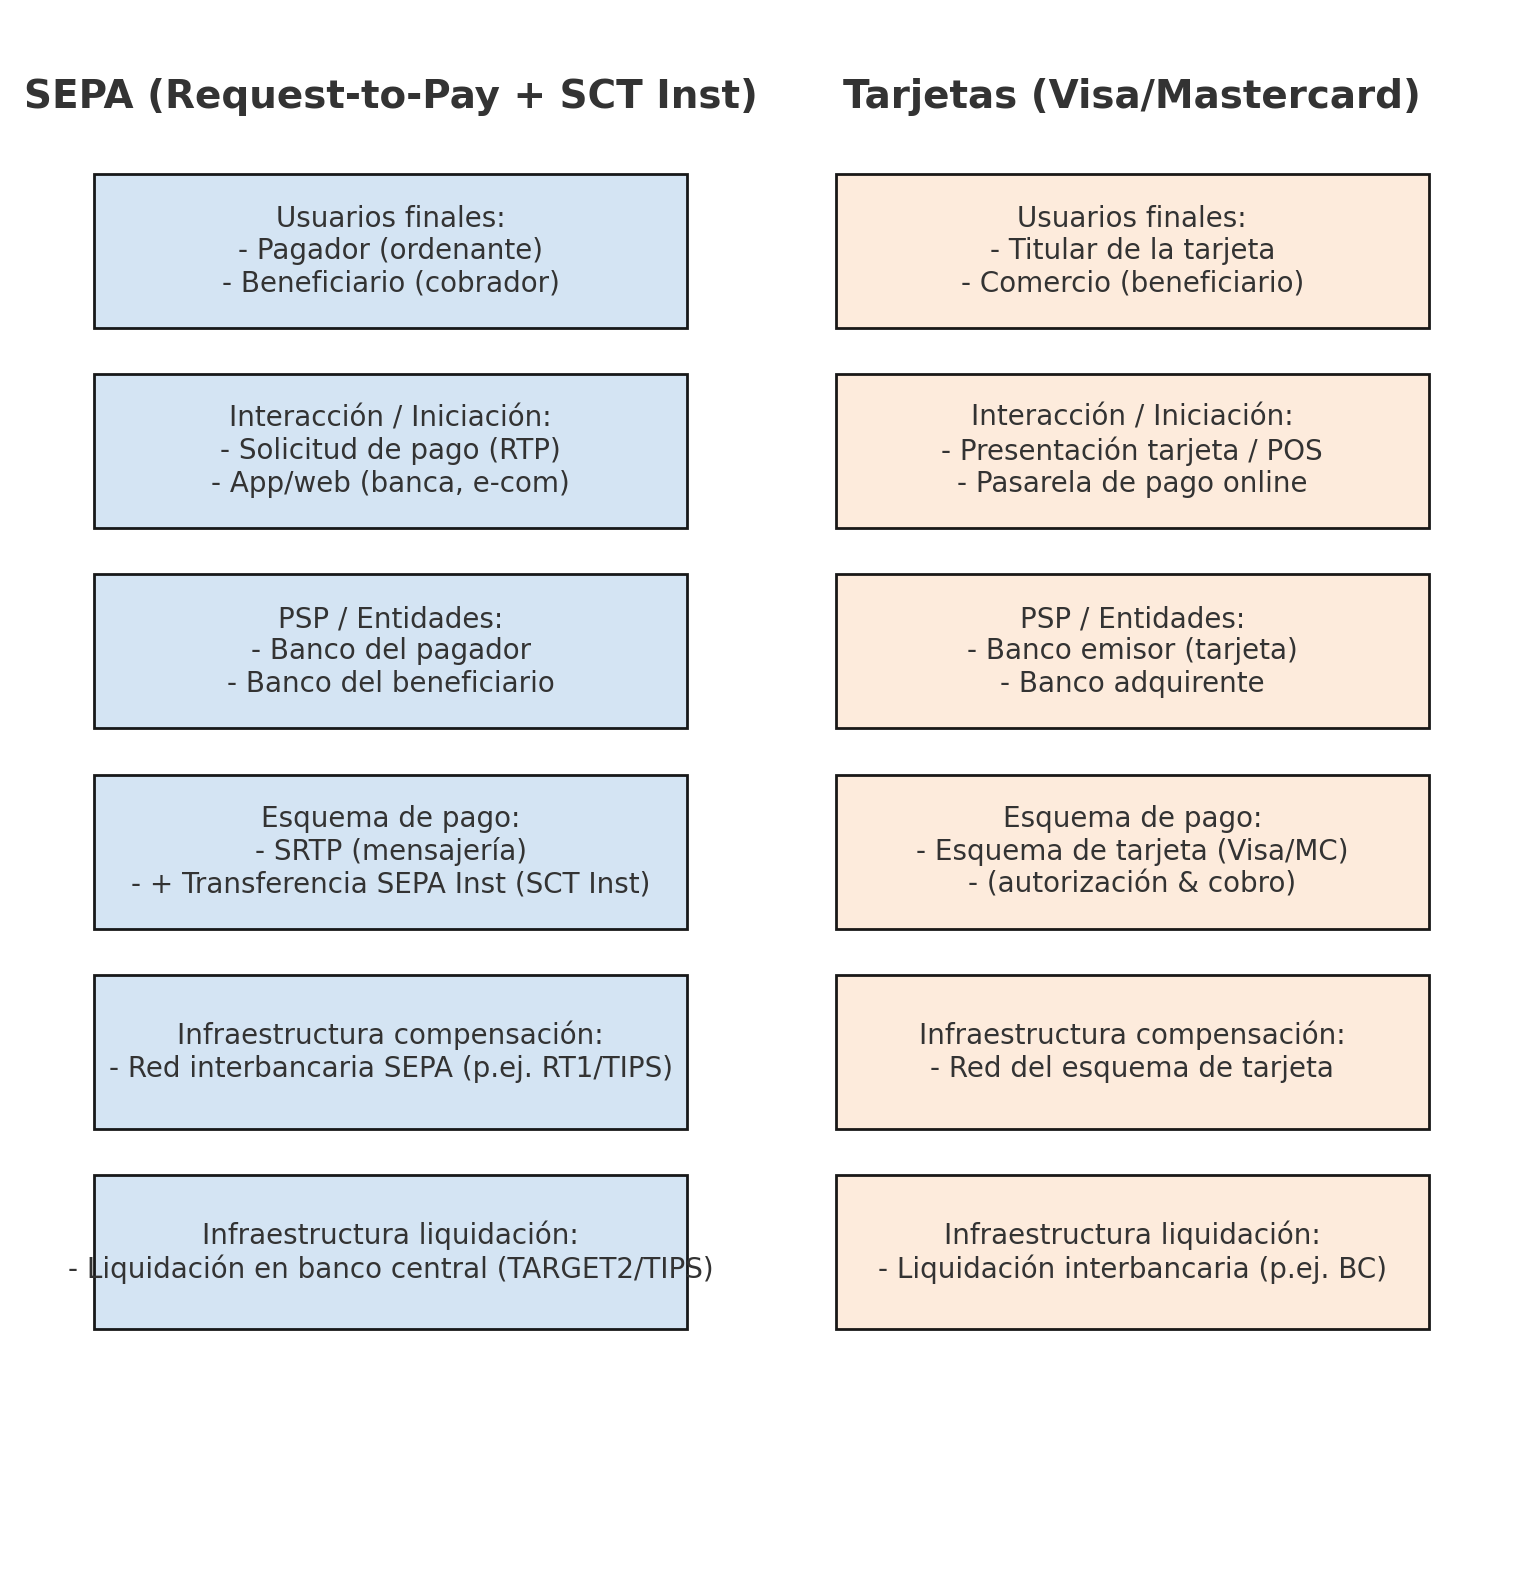
\includegraphics[width=0.8\textwidth]{Imagenes/LayerComp.png}
  \caption{LayerComp}
  \label{fig:Esquema por capas comparación}
\end{figure}

\bigskip

\noindent\textbf{¿Qué simplifica o elimina Request to Pay respecto al modelo de tarjetas?}

Principalmente, elimina intermediarios dedicados y procesos redundantes. Por ejemplo, en un pago SRTP + SCT Inst no es necesario un procesador/acquirente específico ni una red de tarjetas propietaria, ya que los propios bancos de pagador y beneficiario se comunican directamente mediante el esquema común\footnote{\url{https://cpg.de}, \url{https://redbridgedta.com}}. Esto puede reducir costes de aceptación para el comercio (evitando comisiones elevadas de tarjetas) y simplifica la integración: el comercio recibe el dinero directamente en su cuenta bancaria vía SEPA, sin pasos intermedios de recibir fondos a través de entidades de tarjeta y luego liquidarlos. Además, no se requiere que el pagador proporcione datos sensibles como el PAN de tarjeta o incluso su IBAN al comercio; la solicitud llega por canales bancarios seguros y el cliente simplemente autoriza en su entorno bancario\footnote{\url{https://docs.monei.com}}. En resumen, Request to Pay se apoya en la infraestructura bancaria existente (cuentas y pagos inmediatos) para ofrecer una experiencia similar a la de tarjeta, pero con menos capas propietarias, aprovechando la red SEPA ya desplegada en toda Europa.


%----------------------------------------------------------------------
% FIN DE BLOQUE
%----------------------------------------------------------------------


\newpage

% 3. Diseño e Implementación
\section{Diseño e Implementación}
\label{sec:DisenoImplementacion}
Aquí se detalla el proceso de diseño e implementación del servidor HTTP...

\subsection{Arquitectura del servidor HTTP}
\label{subsec:ArquitecturaHTTP}
\subsubsection{Estructura y funcionamiento}
\label{subsubsec:EstructuraFuncionamiento}
El servidor se diseñó para manejar solicitudes y respuestas HTTP de manera eficiente...

\subsubsection{Protocolos y estándares implementados}
\label{subsubsec:Protocolos}
Se implementaron protocolos como HTTP/1.1 y se consideraron estándares de seguridad...

\subsection{Emulación del prototipo \textit{Request To Pay}}
\label{subsec:EmulacionRTP}
\subsubsection{Diseño de las funcionalidades}
\label{subsubsec:DisenoFuncionalidades}
Se replicaron las funcionalidades clave del sistema \textit{Request To Pay}...

\subsubsection{Modelos de procesamiento de solicitudes}
\label{subsubsec:ProcesamientoSolicitudes}
La lógica de negocio se diseñó para procesar solicitudes de pago...

\subsection{Herramientas de desarrollo}
\label{subsec:HerramientasDesarrollo}
\subsubsection{Lenguajes y frameworks}
\label{subsubsec:LenguajesFrameworks}
Se utilizó [especificar lenguaje/framework, e.g., Node.js] para el desarrollo...

\subsubsection{Pruebas y validación}
\label{subsubsec:PruebasValidacion}
Se emplearon herramientas como Postman para validar la funcionalidad del servidor...

\newpage

% 4. Métodos
%\chapter{Métodos}
\label{sec:Metodos}
Esta sección describe los métodos empleados para desarrollar y evaluar el sistema...

\section{Preparación de los datos de entrada}
\label{subsec:PreparacionDatos}
\subsection{Simulación de solicitudes HTTP}
\label{subsubsec:SimulacionSolicitudes}
Se simularon solicitudes HTTP utilizando herramientas como curl...

\subsection{Configuración de escenarios de prueba}
\label{subsubsec:EscenariosPrueba}
Se definieron escenarios de prueba que cubren casos de uso típicos...

\section{Evaluación del sistema}
\label{subsec:EvaluacionSistema}
\subsection{Métricas de rendimiento}
\label{subsubsec:MetricasRendimiento}
Se evaluaron métricas como latencia y \textit{throughput}...

\subsection{Diseño de pruebas}
\label{subsubsec:DisenoPruebas}
Se diseñaron pruebas unitarias, de integración y de carga...

\subsection{Análisis de resultados}
\label{subsubsec:AnalisisResultados}
Los resultados obtenidos se analizaron para identificar cuellos de botella...

\section{Optimización del servidor}
\label{subsec:Optimizacion}
Se implementaron mejoras para optimizar el rendimiento del servidor...

\section{Validación cruzada de la implementación}
\label{subsec:ValidacionCruzada}
La implementación se comparó con los estándares del EPC...

\newpage

% 5. Resultados y discusión
%\chapter{Resultados y discusión}
\label{sec:ResultadosDiscusion}
Esta sección presenta los resultados obtenidos y su análisis...

\section{Presentación de los resultados}
\label{subsec:PresentacionResultados}
\subsection{Comparativa con los estándares del EPC}
\label{subsubsec:ComparativaEPC}
La implementación cumple con los requisitos establecidos por el EPC...

\subsection{Análisis de casos de uso}
\label{subsubsec:AnalisisCasosUso}
Se analizaron casos de uso reales para evaluar el comportamiento del sistema...

\section{Discusión de los resultados}
\label{subsec:DiscusionResultados}
Se discuten las implicaciones de los resultados y las limitaciones encontradas...

\newpage
\chapter{Conclusiones}
\label{sec:Conclusiones}

El desarrollo de este TFG ha representado un esfuerzo significativo que ha culminado en la creación de un prototipo funcional de un servidor HTTP basado en el esquema RTP. El objetivo principal del proyecto —diseñar e implementar un software que simulara las operaciones fundamentales del esquema SEPA RTP utilizando tecnologías actuales y accesibles— se ha alcanzado con éxito. Este trabajo no solo me ha permitido poner en práctica los conocimientos adquiridos durante mi formación en telecomunicaciones y desarrollo de software, sino también explorar un ámbito tan relevante como los sistemas de pago digitales, que desempeñan un papel crucial en la economía global de hoy.

\vspace{0.5cm}

A nivel personal, este TFG ha sido una buena oportunidad para profundizar en el ecosistema SEPA y sus diferentes esquemas de pago. En particular, he podido analizar las limitaciones del SDD y contrastarlas con las ventajas que ofrece RTP. Este aprendizaje no se ha limitado al ámbito teórico: la implementación práctica del prototipo me ha enfrentado a retos técnicos que han fortalecido mis competencias como desarrollador.

\vspace{0.5cm}

El proceso de desarrollo también ha sido una lección sobre la importancia de una metodología bien definida, lo que me permitió avanzar de manera constante, detectar errores a tiempo y ajustar los objetivos según las necesidades del proyecto. Este enfoque estructurado, combinado con una documentación detallada de cada etapa, ha sido clave para mantener el control sobre el proyecto.
\vspace{0.5cm}


El sistema RTP se posiciona como un candidato ideal paraq convertirse en un estándar en la zona SEPA, especialmente a medida que más instituciones financieras y PSP adopten el esquema y lo integren en sus operaciones. En el futuro, es probable que RTP no solo facilite los pagos entre empresas y consumidores, sino que también fomente una mayor interoprabilidad y eficiencia en el mercado financiaro europeo, contribuyendo a una economía más conectada y dinámica.
\vspace{0.5cm}

\newpage
\null
\clearpage
\chapter{Líneas futuras}
\label{sec:Potencial}
En cuanto al prototipo desarollado, aunque satisface plenamente los objetivos establecidos para este TFG, su potencial va mucho más allá de un simple ejercicio acádemico. Durante el proceso identifiqué varias áreas de mejora que podrían transformar este simulador en una herramienta aplicable en escenarios reales. A continuación, detallo algunas de estas oportunidades de evolución:

\begin{enumerate}
    \item \textbf{Escalabilidad del sistema:} La base de datos SQLite, aunque suficiente para un prototipo, tiene limitaciones en térmninos de rendimiento y capacidad. Para soportar un mayor volumen de usuarios y transacciones, sería necesario migrar a un sistema más robusto como PostgreSQL o MySQL, que ofrecen mejor escalabilidad y soporte para entornos de producción.
    \item \textbf{Fortalecimiento de la seguridad:} El prototipo incluye medidas básicas de autenticación, pero un sistema real requeriría estándares más altos, como la encriptación de extremo a extremo, autenticación multifactor y cumplimiento con normativas como PSD2 (Payment Services Directive 2) y GDPR (General Data Protection Regulation). Estas mejoras garantizarían la protección de los datos sensibles y la confianza de los usuarios.
    \item \textbf{Interoperabilidad con sistemas bancarios:} Para que el prototipo trascienda su estado actual, sería esencial integrarlo con las APIs de bancos y PSP reales. Esto permitiría ejecutar transacciones monetarias auténticas y demostrar su utilidad en un contexto práctico, un paso crítico hacia su adopción en el mundo real.
    \item \textbf{Ampliación de funcionalidades:} El sistema podría enriquecerse con características avanzadas, como soporte para pagos recurrentes (ideal para suscripciones o facturas periódicas), compatibilidad con múltiples monedas (facilitando transacciones transfronterizas), herramientas analíticas que ofrezcan estadísticas a los usuarios, y reportes detallados sobre el historial de pagos. Estas adiciones harían que el sistema fuera más versátil y atractivo para distintos tipos de usuarios.
    \item \textbf{Mejora de la experiencia de usario:} Aunque el frontend actual es funcional, podría optimizarse con un diseño más moderno y accesible. Incorporar elementos como notificaciones push, un historial visual de transacciones, opciones de personalización y una interfaz adaptada a dispositivos móviles elevaría la usabilidad y la satisfacción del usuario.
\end{enumerate}

Estas mejoras, aunque son algo ambiciosas, son alcanzables con el tiempo y los recursos adecuados. Implementarlas no solo incrementaría la funcionalidad del prototipo, sino que también lo alinearía con las demandas de un mercado financiero en constante camnbio, donde la innovación y la adaptabilidad son esenciales.
\vspace{0.5cm}
\newpage
% Añadiendo los apéndices
\clearpage


% Añadiendo las referencias
\clearpage
\renewcommand{\bibname}{Referencias}
\bibliographystyle{castellano2}
\bibliography{bibliografia}

% Añadiendo el índice de figuras
\newpage
\renewcommand{\listfigurename}{Índice de Figuras}
\listoffigures
\addcontentsline{toc}{section}{Índice de Figuras}

% Añadiendo el índice de tablas
\newpage
\renewcommand{\listtablename}{Índice de Tablas}
\listoftables
\addcontentsline{toc}{section}{Índice de Tablas}

% Añadiendo el índice de códigos
\newpage
\renewcommand*{\lstlistlistingname}{Índice de Códigos}
\renewcommand*{\lstlistingname}{Código}
\lstlistoflistings
\addcontentsline{toc}{section}{Índice de Códigos}

\end{document}